\documentclass{article}\usepackage[]{graphicx}\usepackage[]{color}
%% maxwidth is the original width if it is less than linewidth
%% otherwise use linewidth (to make sure the graphics do not exceed the margin)
\makeatletter
\def\maxwidth{ %
  \ifdim\Gin@nat@width>\linewidth
    \linewidth
  \else
    \Gin@nat@width
  \fi
}
\makeatother

\definecolor{fgcolor}{rgb}{0.345, 0.345, 0.345}
\newcommand{\hlnum}[1]{\textcolor[rgb]{0.686,0.059,0.569}{#1}}%
\newcommand{\hlstr}[1]{\textcolor[rgb]{0.192,0.494,0.8}{#1}}%
\newcommand{\hlcom}[1]{\textcolor[rgb]{0.678,0.584,0.686}{\textit{#1}}}%
\newcommand{\hlopt}[1]{\textcolor[rgb]{0,0,0}{#1}}%
\newcommand{\hlstd}[1]{\textcolor[rgb]{0.345,0.345,0.345}{#1}}%
\newcommand{\hlkwa}[1]{\textcolor[rgb]{0.161,0.373,0.58}{\textbf{#1}}}%
\newcommand{\hlkwb}[1]{\textcolor[rgb]{0.69,0.353,0.396}{#1}}%
\newcommand{\hlkwc}[1]{\textcolor[rgb]{0.333,0.667,0.333}{#1}}%
\newcommand{\hlkwd}[1]{\textcolor[rgb]{0.737,0.353,0.396}{\textbf{#1}}}%

\usepackage{framed}
\makeatletter
\newenvironment{kframe}{%
 \def\at@end@of@kframe{}%
 \ifinner\ifhmode%
  \def\at@end@of@kframe{\end{minipage}}%
  \begin{minipage}{\columnwidth}%
 \fi\fi%
 \def\FrameCommand##1{\hskip\@totalleftmargin \hskip-\fboxsep
 \colorbox{shadecolor}{##1}\hskip-\fboxsep
     % There is no \\@totalrightmargin, so:
     \hskip-\linewidth \hskip-\@totalleftmargin \hskip\columnwidth}%
 \MakeFramed {\advance\hsize-\width
   \@totalleftmargin\z@ \linewidth\hsize
   \@setminipage}}%
 {\par\unskip\endMakeFramed%
 \at@end@of@kframe}
\makeatother

\definecolor{shadecolor}{rgb}{.97, .97, .97}
\definecolor{messagecolor}{rgb}{0, 0, 0}
\definecolor{warningcolor}{rgb}{1, 0, 1}
\definecolor{errorcolor}{rgb}{1, 0, 0}
\newenvironment{knitrout}{}{} % an empty environment to be redefined in TeX

\usepackage{alltt}
\usepackage{amscd, amssymb, amsmath, verbatim, setspace}
\usepackage[left=1.0in, right=1.0in, top=1.0in, bottom=1.0in]{geometry}
\usepackage{mathrsfs}
\usepackage{listings}


\IfFileExists{upquote.sty}{\usepackage{upquote}}{}
\begin{document}

\begin{flushright}
  Arif Ali\\
  ANLY-511 Prob. Modeling \& Stat. Computing\\
	Dec 21, 2015\\
\end{flushright}

\begin{center}
  \LARGE\textbf{Take Home Examination}
\end{center}
\begin{knitrout}
\definecolor{shadecolor}{rgb}{1, 1, 1}\color{fgcolor}\begin{kframe}
\begin{verbatim}
load("~/Dropbox/School/Georgetown/Analytics 511 Fall 2015/final.rdata")
\end{verbatim}
\end{kframe}
\end{knitrout}

\section*{Problem 1}
Given that $X_{1}$ and $X_{2}$ are independent of one another, we are able to use the properties of Expectation and variance in the case of indepedence which is $E(Y)=E(X_{1})+E(X_{2})$ and $Var(Y)=Var(X_{1})+Var(X_{2})$. Since, we know that both $\sigma$ and $\lambda$ are whole numbers, the exact values should be rounded values of the the sample values. 
\begin{knitrout}
\definecolor{shadecolor}{rgb}{1, 1, 1}\color{fgcolor}\begin{kframe}
\begin{verbatim}
mean(problem1)
## [1] 6.238424
var(problem1)
## [1] 14.77133
\end{verbatim}
\end{kframe}
\end{knitrout}

\begin{equation}
E(Y)=E(X_{1})+E(X_{2})=0+\hat\lambda=6.238424 \implies \lambda = 6
\end{equation}

\begin{equation}
Var(Y)=Var(X_{1})+Var(X_{2})=\hat\sigma^2+\hat\lambda=14.77 \implies \hat\sigma^2 = 14.77 - 6.24 = 8.53 \implies \sigma = 3
\end{equation}

\section*{Problem 2}
\subsection*{Part A}
\begin{knitrout}
\definecolor{shadecolor}{rgb}{1, 1, 1}\color{fgcolor}\begin{kframe}
\begin{verbatim}
Nevada = handle.times[handle.times$program=="Nevada","time"]
hist(Nevada)
qqnorm(Nevada)
qqline(Nevada)
bootstrap.ne = replicate(10000, mean(sample(Nevada, 
                                            length(Nevada), 
                                            replace = T)))
# 95% Confidence Interval:
quantile(bootstrap.ne, c(0.025,0.975))
##     2.5%    97.5% 
## 453.8555 531.3701
\end{verbatim}
\end{kframe}
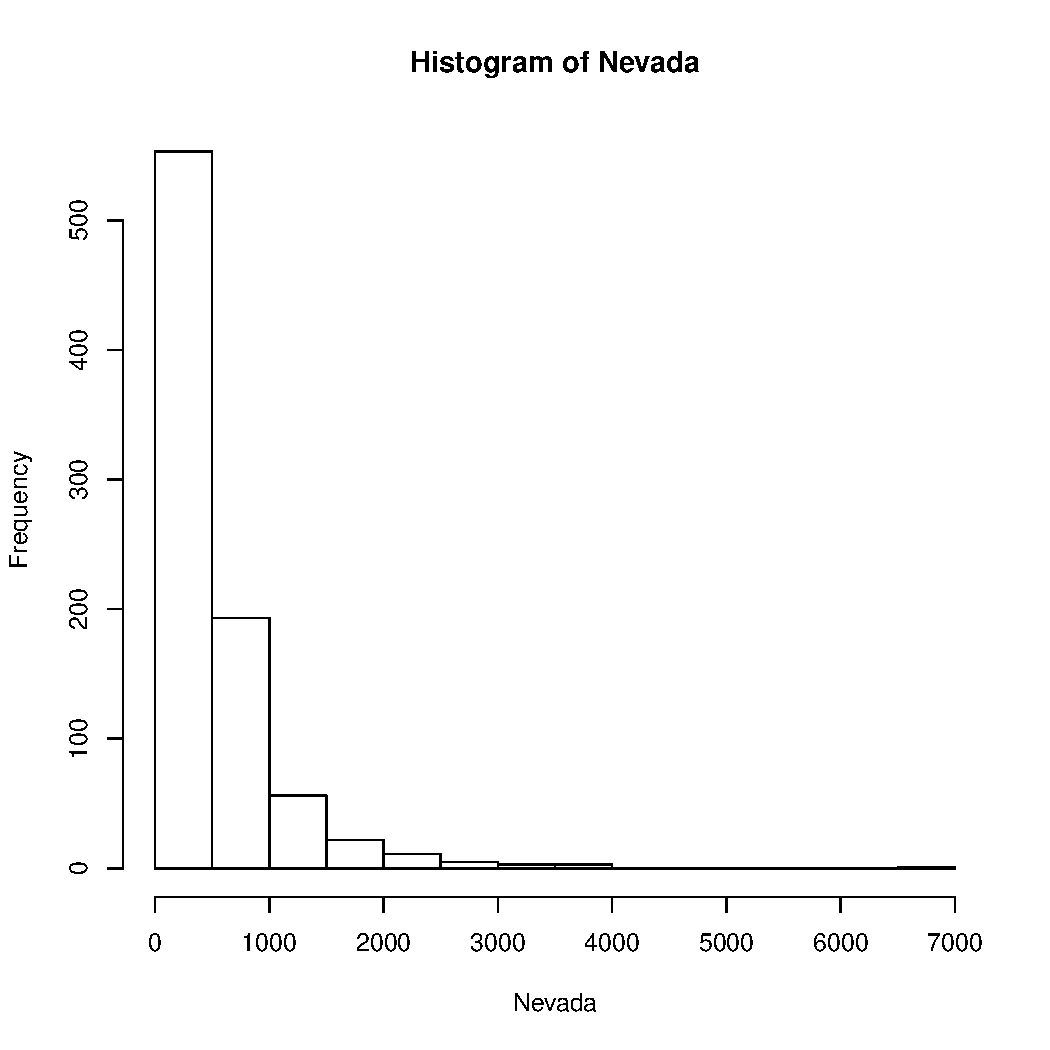
\includegraphics[width=0.33\linewidth]{figure/unnamed-chunk-4-1} 
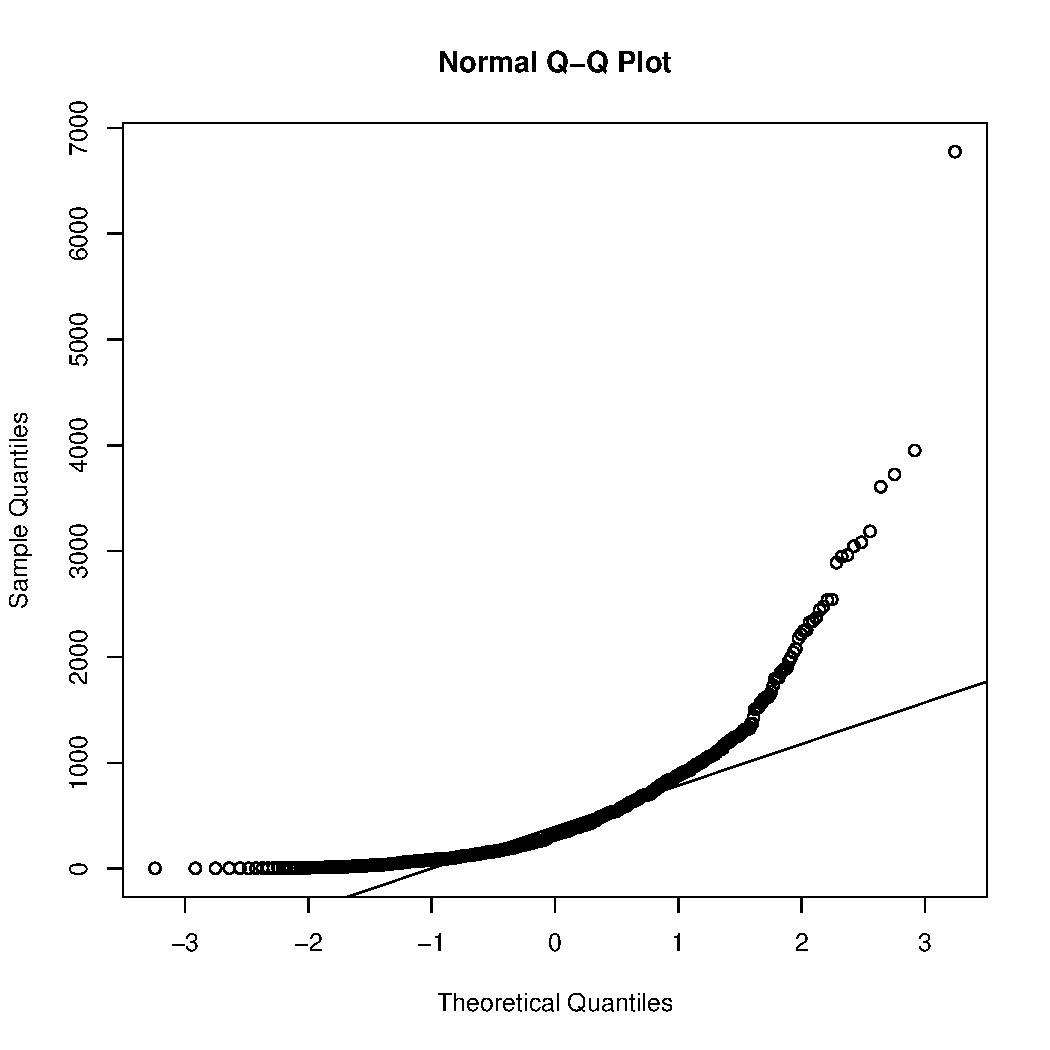
\includegraphics[width=0.33\linewidth]{figure/unnamed-chunk-4-2} 

\end{knitrout}
Using the z-statistic method, requires knowing the mean and variance of the entire population relative to a sample. The t-statistic confidence interval method assumes that $\mu$ is the sample mean and that we can the sample standard deviation. However, this method also assumes that the sample should follow close the normal distribution. Based on the histogram and qqnorm plot, it is clear that this is not the case. Given out skewed the data is, the bootstrap method for the confidence interval is better compared the the t-statistic or z-statistic (normal method).
\subsection*{Part B}
$H_{0}:\mu=540$
$H_{a}:\mu<540$
\begin{knitrout}
\definecolor{shadecolor}{rgb}{1, 1, 1}\color{fgcolor}\begin{kframe}
\begin{verbatim}
WB = handle.times[handle.times$program=="West Billing","time"]
hist(WB, breaks = 20)
qqnorm(WB); qqline(WB);
E2b = replicate(10000, mean(sample(WB, length(WB), replace = T)))

#P-value
mean(E2b>=540)
## [1] 0.0021
\end{verbatim}
\end{kframe}
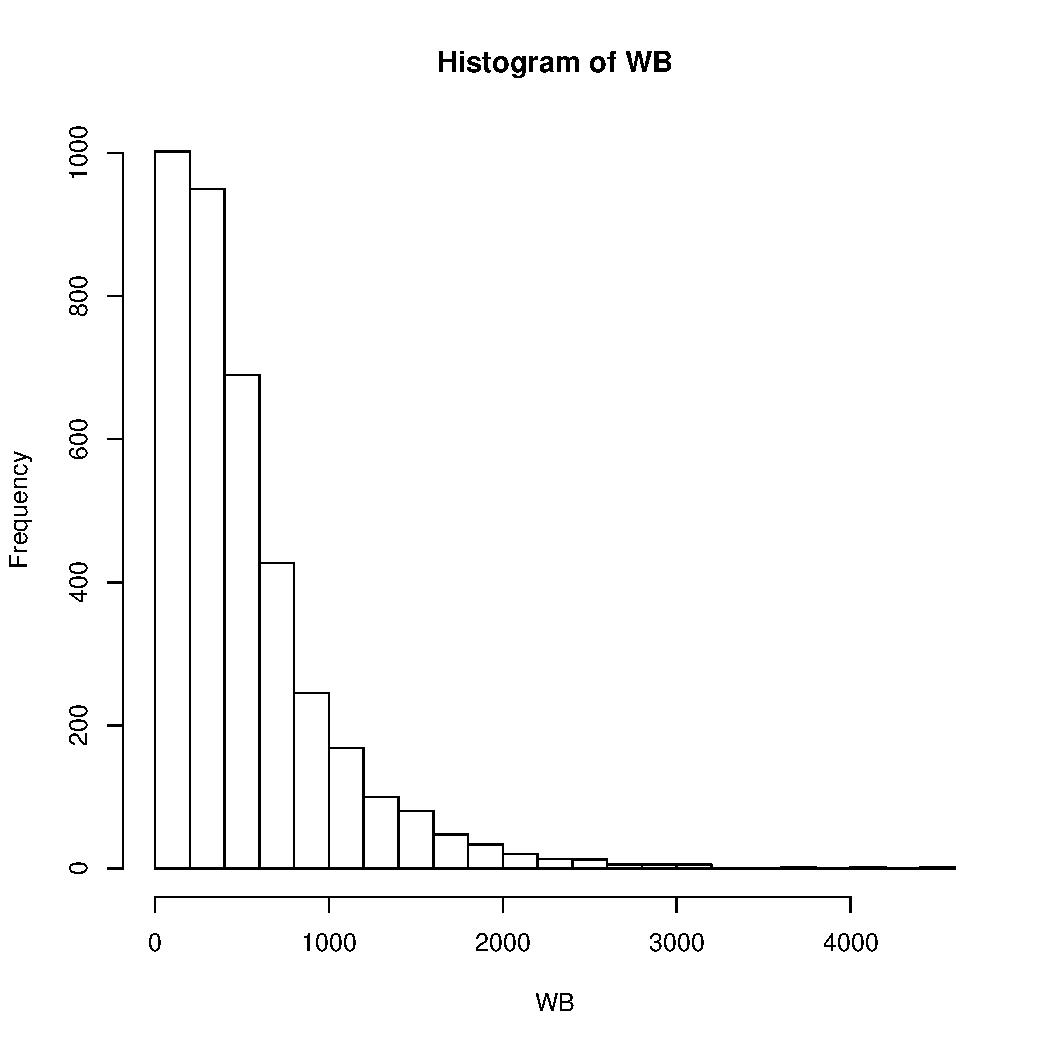
\includegraphics[width=0.33\linewidth]{figure/unnamed-chunk-5-1} 
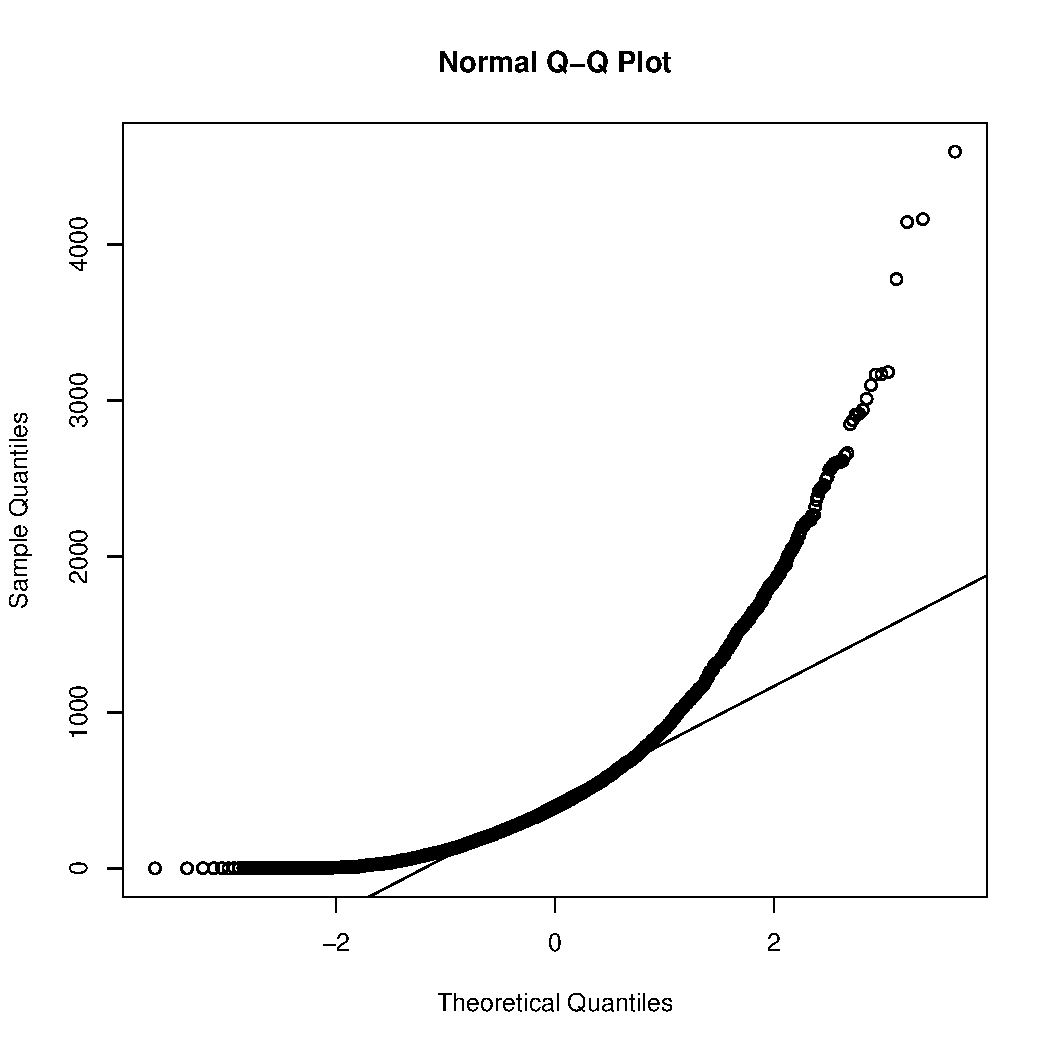
\includegraphics[width=0.33\linewidth]{figure/unnamed-chunk-5-2} 

\end{knitrout}
The t test assumes that the data is somewhat normal; however, based on the histogram and the qqnorm plots, it is clear that the data is not normal and skewed to the left. Therefore, the best idea is too see permutations of WB by sampling them with replacement and determining the mean. Based on the p-value, we reject the null hypothesis that mean of handle times for West Billing is 540 in favor of the alternative hypothesis, that handle times are less than 540 seconds.  
\subsection*{Part C}
\begin{knitrout}
\definecolor{shadecolor}{rgb}{1, 1, 1}\color{fgcolor}\begin{kframe}
\begin{verbatim}
LD = handle.times[handle.times$program=="LD Care","time"]
hist(LD, breaks = 20)
qqnorm(LD); qqline(LD);

LD.WB = function(){
  l.sample = mean(sample(LD, length(LD), replace = T))
  w.sample = mean(sample(WB, length(WB), replace = T))
  return(l.sample-w.sample)
}
lw.bootstrap = replicate(10000, LD.WB())

# 90% Confidence Interval:
quantile(lw.bootstrap, c(0.05,0.95))
##        5%       95% 
## -423.9365  139.2426
\end{verbatim}
\end{kframe}
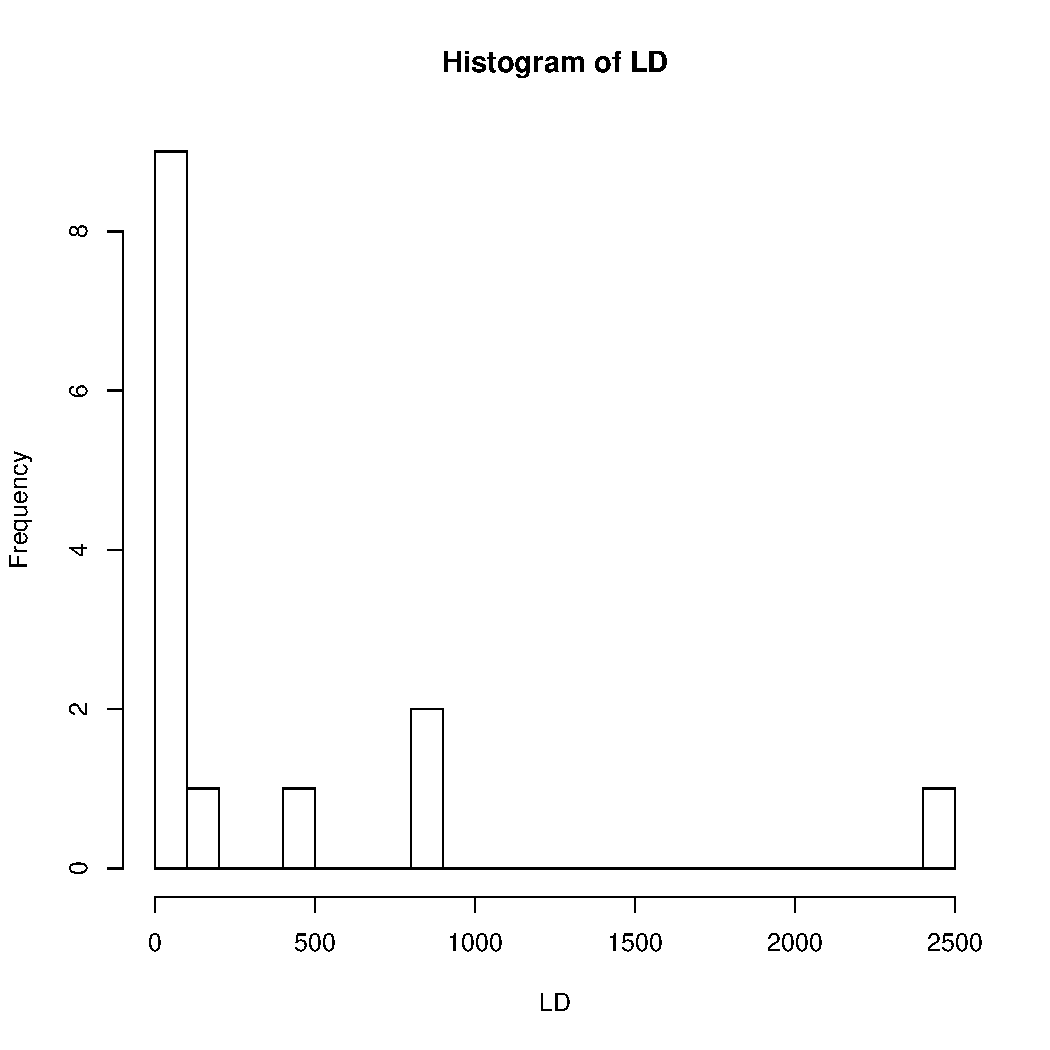
\includegraphics[width=0.33\linewidth]{figure/unnamed-chunk-6-1} 
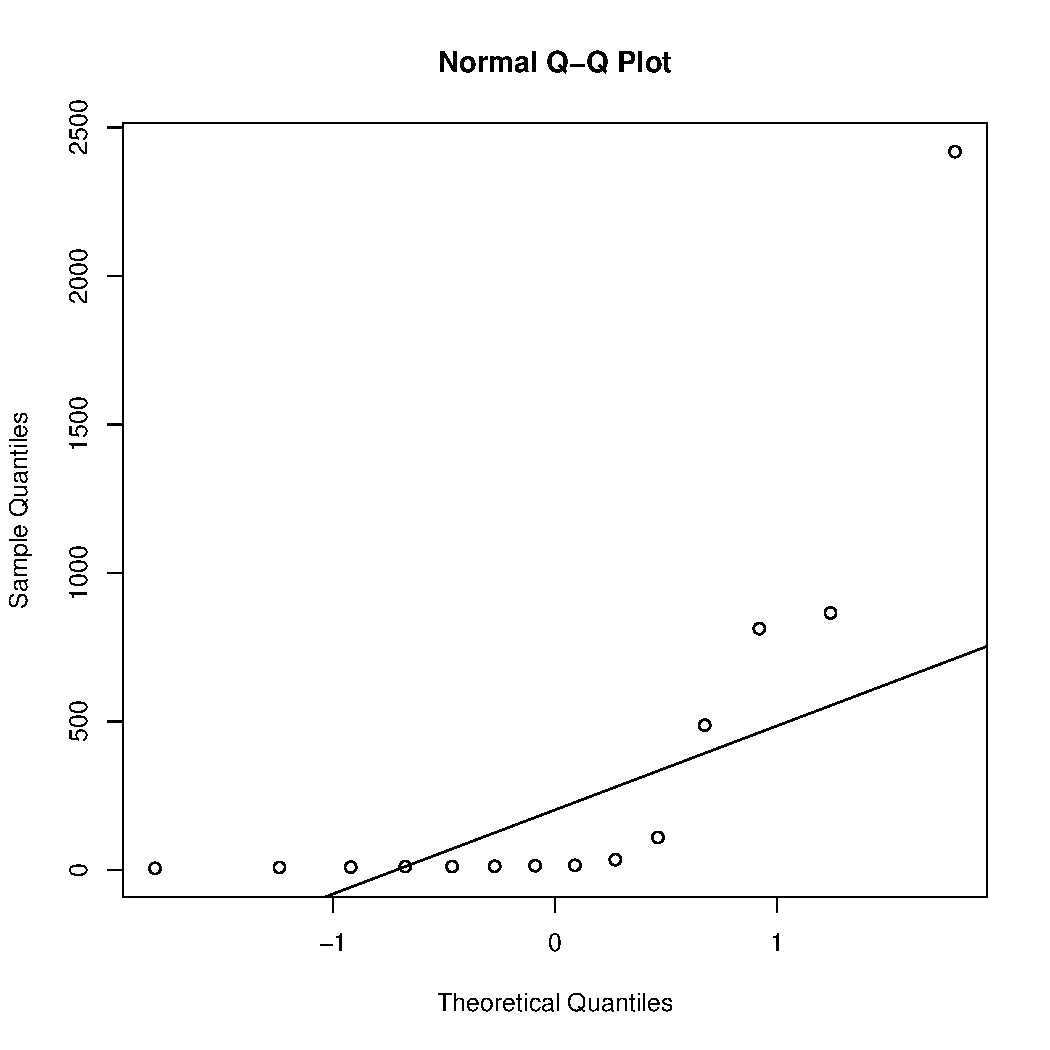
\includegraphics[width=0.33\linewidth]{figure/unnamed-chunk-6-2} 

\end{knitrout}
Neither of the samples follow close to a normal distribution, so both the the z and t statistics methods for building a confidence interval is not appropriate. Based on the histogram, both samples are very skewed, so it seems to be best to apply the bootstrap method for the confidence interval. 
\section*{Problem 3}
\subsection*{Part A}
\begin{knitrout}
\definecolor{shadecolor}{rgb}{1, 1, 1}\color{fgcolor}\begin{kframe}
\begin{verbatim}
Part3ai = replicate(10000,sum(rpois(n = 20, lambda = 10)))
alpha = 0.05
qqnorm(Part3ai)
qqline(Part3ai)
\end{verbatim}
\end{kframe}
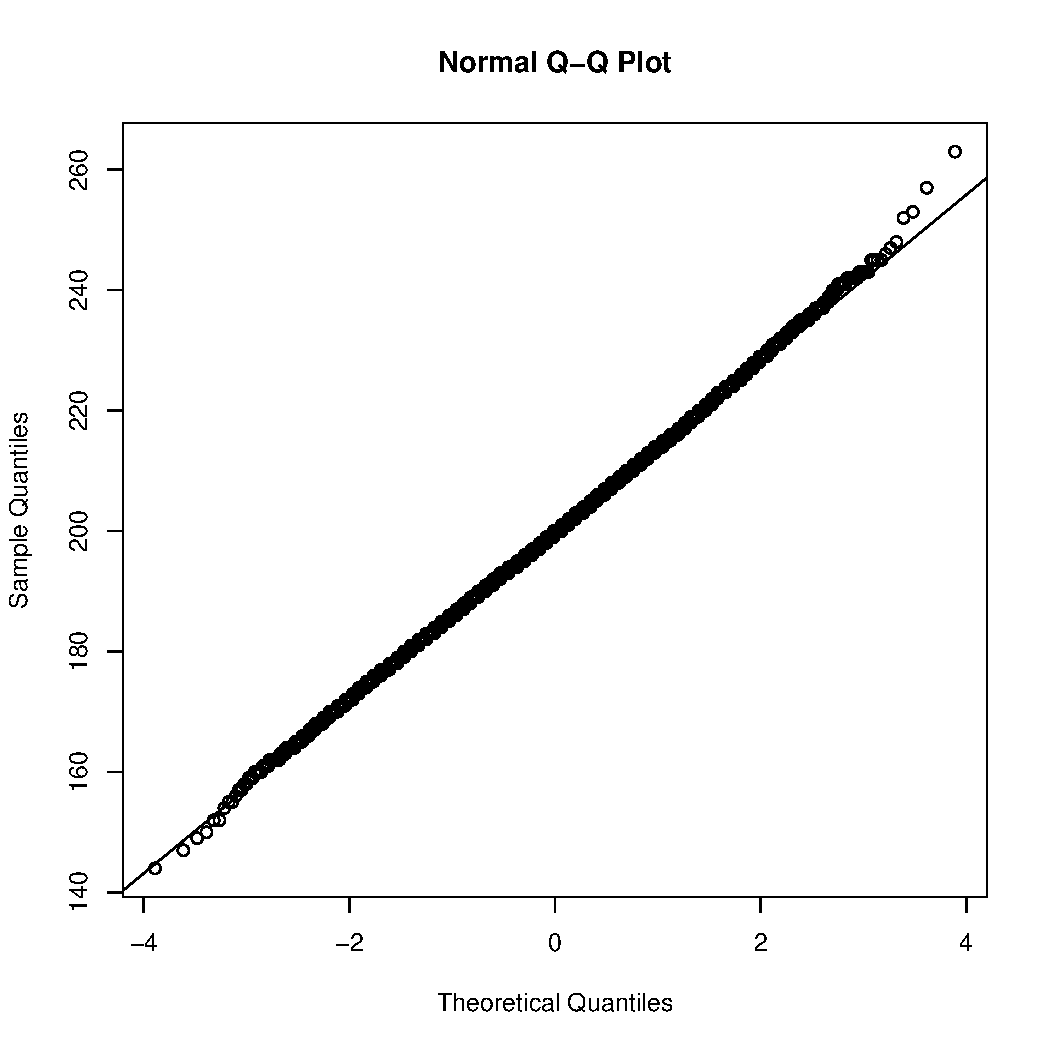
\includegraphics[width=0.33\linewidth]{figure/unnamed-chunk-7-1} 
\begin{kframe}\begin{verbatim}
c1 = qnorm(1-alpha, mean(Part3ai), sd(Part3ai))
c1
## [1] 222.9913
Part3aii = replicate(10000,max(rpois(n = 20, lambda = 10)))
qqnorm(Part3aii)
qqline(Part3aii)
\end{verbatim}
\end{kframe}
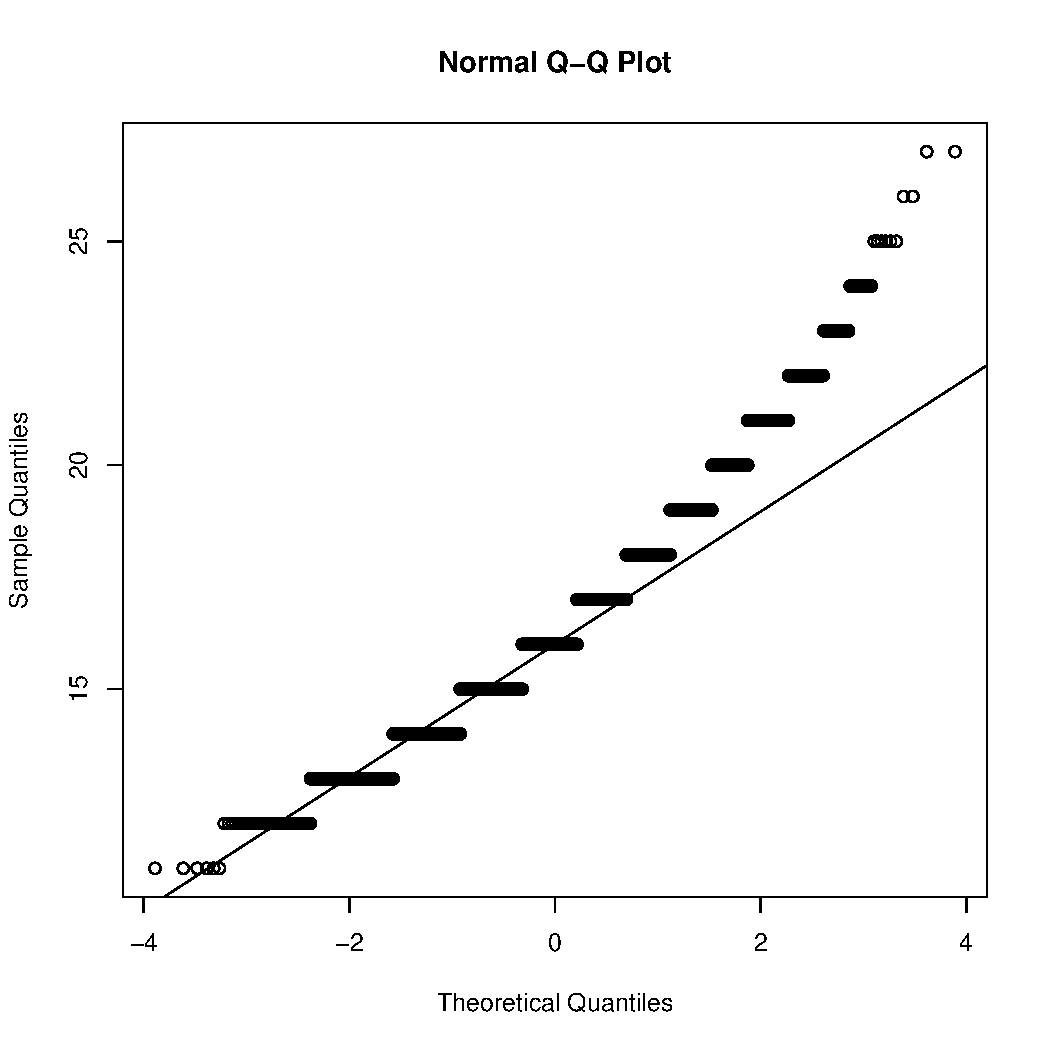
\includegraphics[width=0.33\linewidth]{figure/unnamed-chunk-7-2} 
\begin{kframe}\begin{verbatim}
sample.poisson = rpois(n = 1000, lambda = 10)
qqnorm(sample.poisson)
qqline(sample.poisson)
\end{verbatim}
\end{kframe}
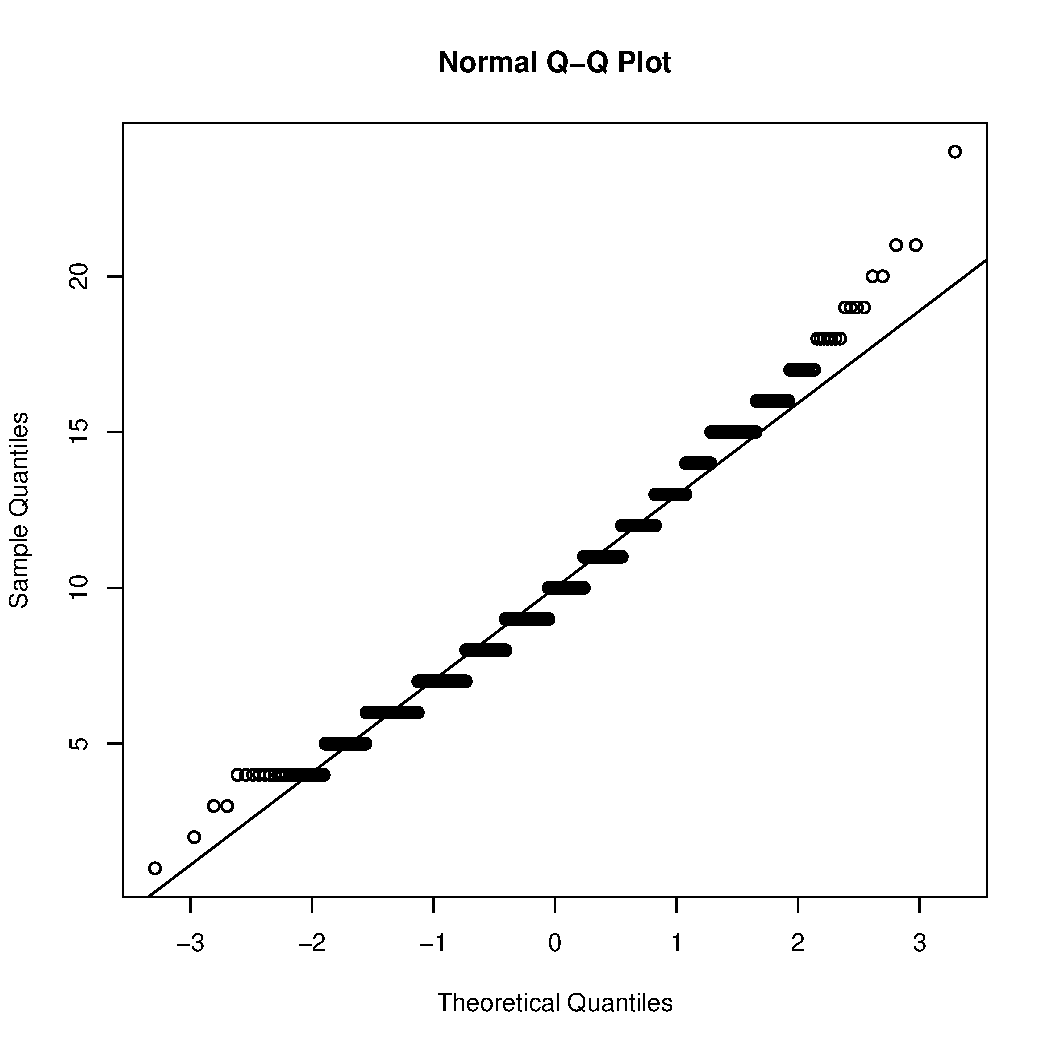
\includegraphics[width=0.33\linewidth]{figure/unnamed-chunk-7-3} 
\begin{kframe}\begin{verbatim}
c2 = qpois(1-alpha, mean(Part3aii))
c2
## [1] 23
\end{verbatim}
\end{kframe}
\end{knitrout}
The replications for both $T_{1}$ and $T_{2}$ was done 10000 times in order to simulate the various values. In order to properly $T_{1}$ and $T_{2}$, I replicated both methods using rpois to generate the values of $x_1, x_2,...,x_{20}$. For $T_{2}$, the assumption of normality cannot hold. This is confirmed by the qqnorm plot which shows a step like structure. This structure is similar to a qqnorm of numbers generated from a poisson distribution. Therefore, for $c_{2}$, the best approach to estimating is using the qpois approach.           
\subsection*{Part B}
With the $T_{1}$ Test:
\begin{knitrout}
\definecolor{shadecolor}{rgb}{1, 1, 1}\color{fgcolor}\begin{kframe}
\begin{verbatim}
Part3bi = replicate(10000,sum(rpois(n = 20, lambda = 15)))
hist(Part3ai, xlim = c(min(Part3ai), max(Part3bi)), breaks = 50, col = "#4C0CE8", main = "T1")
hist(Part3bi, breaks = 50, add = T, col = "#FF00A8A6")
abline(v = c1, col = 'red')
\end{verbatim}
\end{kframe}
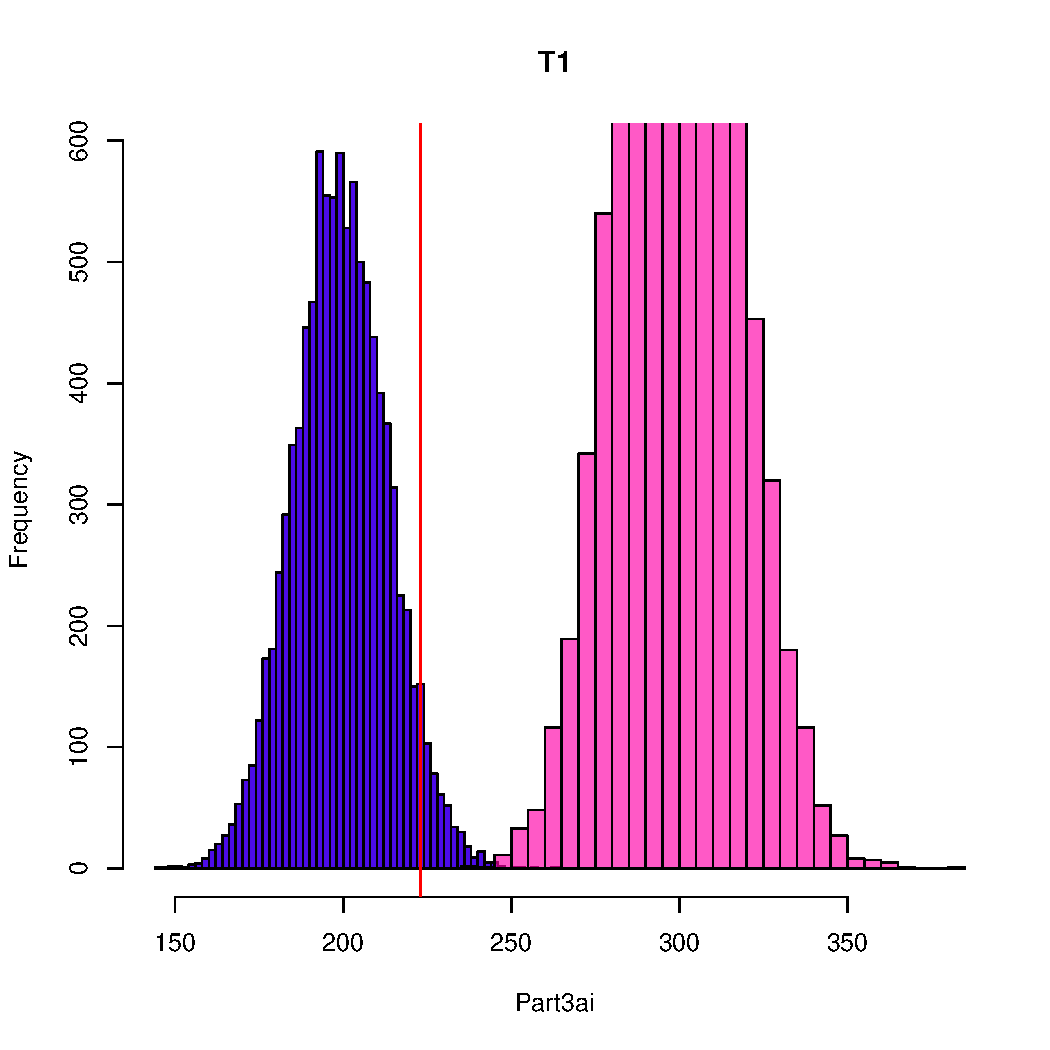
\includegraphics[width=0.33\linewidth]{figure/unnamed-chunk-8-1} 
\begin{kframe}\begin{verbatim}
# Type II error:
pnorm(c1, mean(Part3bi), sd(Part3bi))
## [1] 3.612225e-06
\end{verbatim}
\end{kframe}
\end{knitrout}
The Histogram shows the data from the two simulations next to one another. The second histogram is transparent to show where the graphs overlap. The line represents where $c_1$ is in relation to both simulations. It's interesting to see that $c_1$ appears to not occur at any point of the histogram based on $\lambda = 15$. Running the pnorm gives the probability of this ever occuring. The value is so small, so the Type II error is very small, which means that the Power of the test is large.  
With the $T_{2}$ Test:
\begin{knitrout}
\definecolor{shadecolor}{rgb}{1, 1, 1}\color{fgcolor}\begin{kframe}
\begin{verbatim}
Part3bii = replicate(10000,max(rpois(n = 20, lambda = 15)))
hist(Part3aii, xlim = c(min(Part3aii), max(Part3bii)), breaks = 20, col = "#4C0CE8", main = "T2")
hist(Part3bii, breaks = 20, add = T, col = "#FF00A8A6")
abline(v = c2, col = 'red')
\end{verbatim}
\end{kframe}
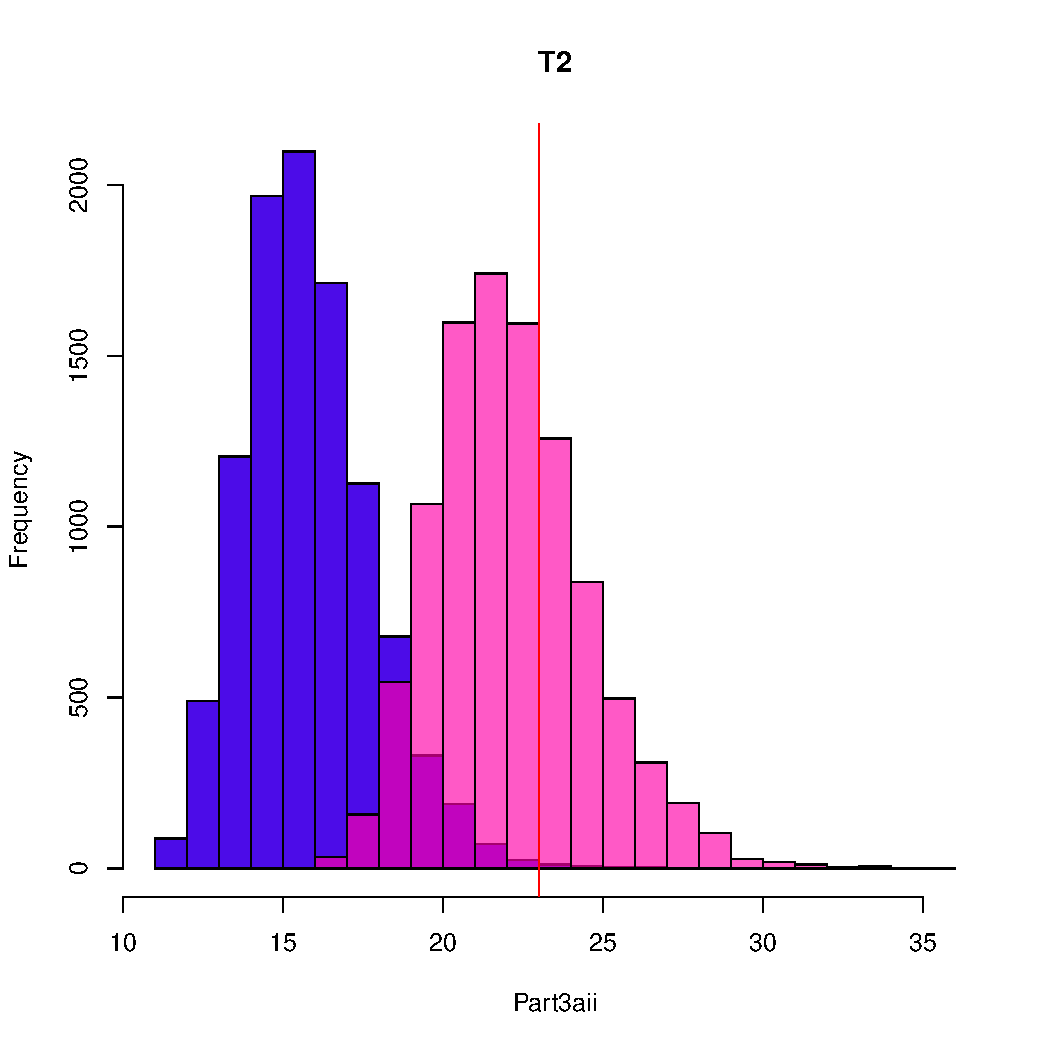
\includegraphics[width=0.33\linewidth]{figure/unnamed-chunk-9-1} 
\begin{kframe}\begin{verbatim}
# Type II error:
ppois(c2, mean(Part3bii))
## [1] 0.5843319
\end{verbatim}
\end{kframe}
\end{knitrout}
The same logic behind the histogram from $T_{1}$ was the same that was applied to $T_{2}$ using ppois instead of pnorm, but the line represents where $c_{2}$ is capturing more of the distribution generated from $\lambda=15$. Unlike the histograms for $T_{1}$, there is noticable overlap between the two histograms. The value of the type II is larger for $T_{2}$ as opposed to $T_{1}$. 
\subsection*{Bonus}
Using the $T_{1}$ Test:
\begin{knitrout}
\definecolor{shadecolor}{rgb}{1, 1, 1}\color{fgcolor}\begin{kframe}
\begin{verbatim}
Part3bonusi = replicate(10000,sum(rpois(n = 20, lambda = 8)))
hist(Part3bonusi, xlim = c(min(Part3bonusi), max(Part3ai)), breaks = 50, col = "#4C0CE8", main = "T1")
hist(Part3ai, breaks = 50, add = T, col = "#FF00A8A6")
abline(v = c1, col = 'red')
\end{verbatim}
\end{kframe}
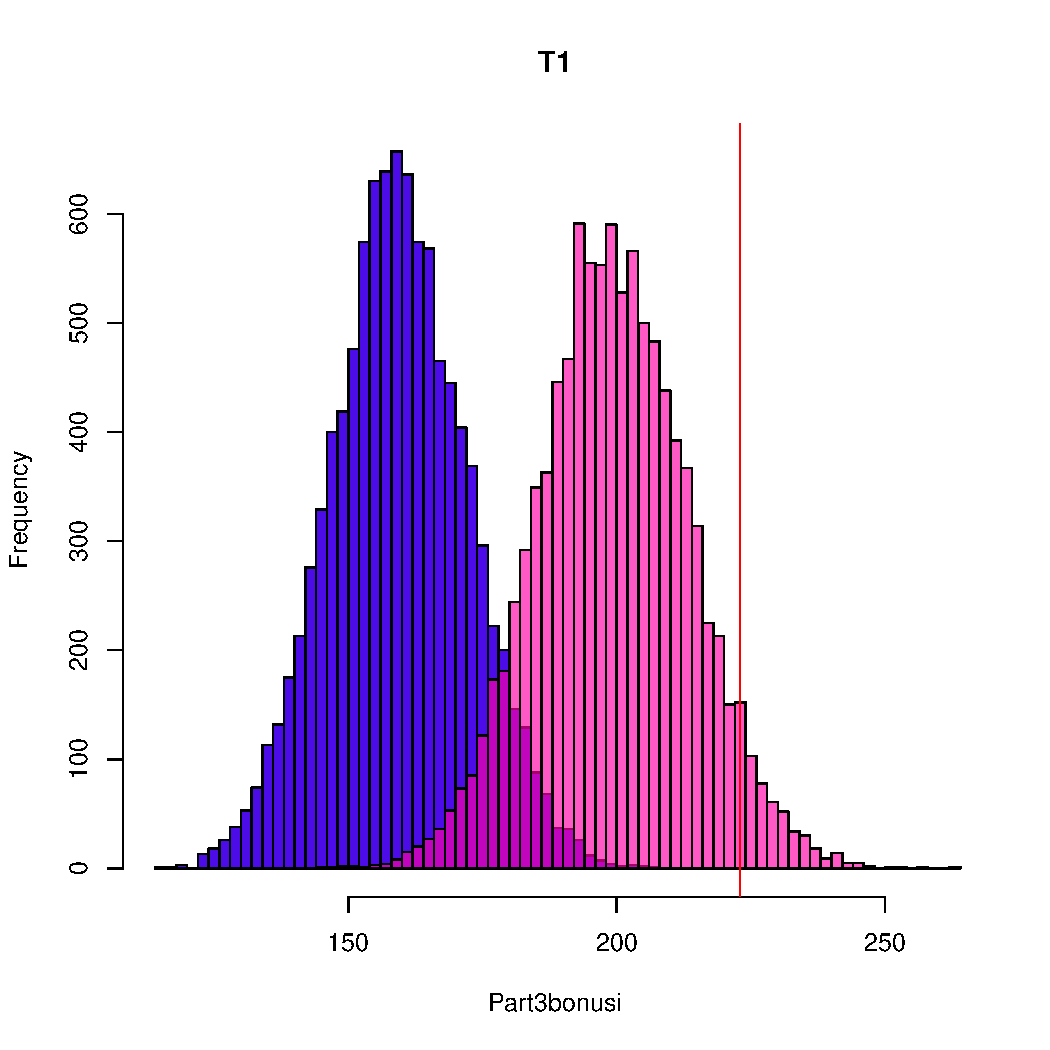
\includegraphics[width=0.33\linewidth]{figure/unnamed-chunk-10-1} 
\begin{kframe}\begin{verbatim}
# Probability of rejecting H0:
pnorm(c1, mean(Part3bonusi), sd(Part3bonusi), lower.tail = F)
## [1] 3.985083e-07
\end{verbatim}
\end{kframe}
\end{knitrout}

Using the $T_{2}$ Test:
\begin{knitrout}
\definecolor{shadecolor}{rgb}{1, 1, 1}\color{fgcolor}\begin{kframe}
\begin{verbatim}
Part3bonusii = replicate(10000,max(rpois(n = 20, lambda = 8)))
hist(Part3bonusii, xlim = c(min(Part3bonusii), max(Part3aii)), breaks = 20, col = "#4C0CE8", main = "T1")
hist(Part3aii, breaks = 20, add = T, col = "#FF00A8A6")
abline(v = c2, col = 'red')
\end{verbatim}
\end{kframe}
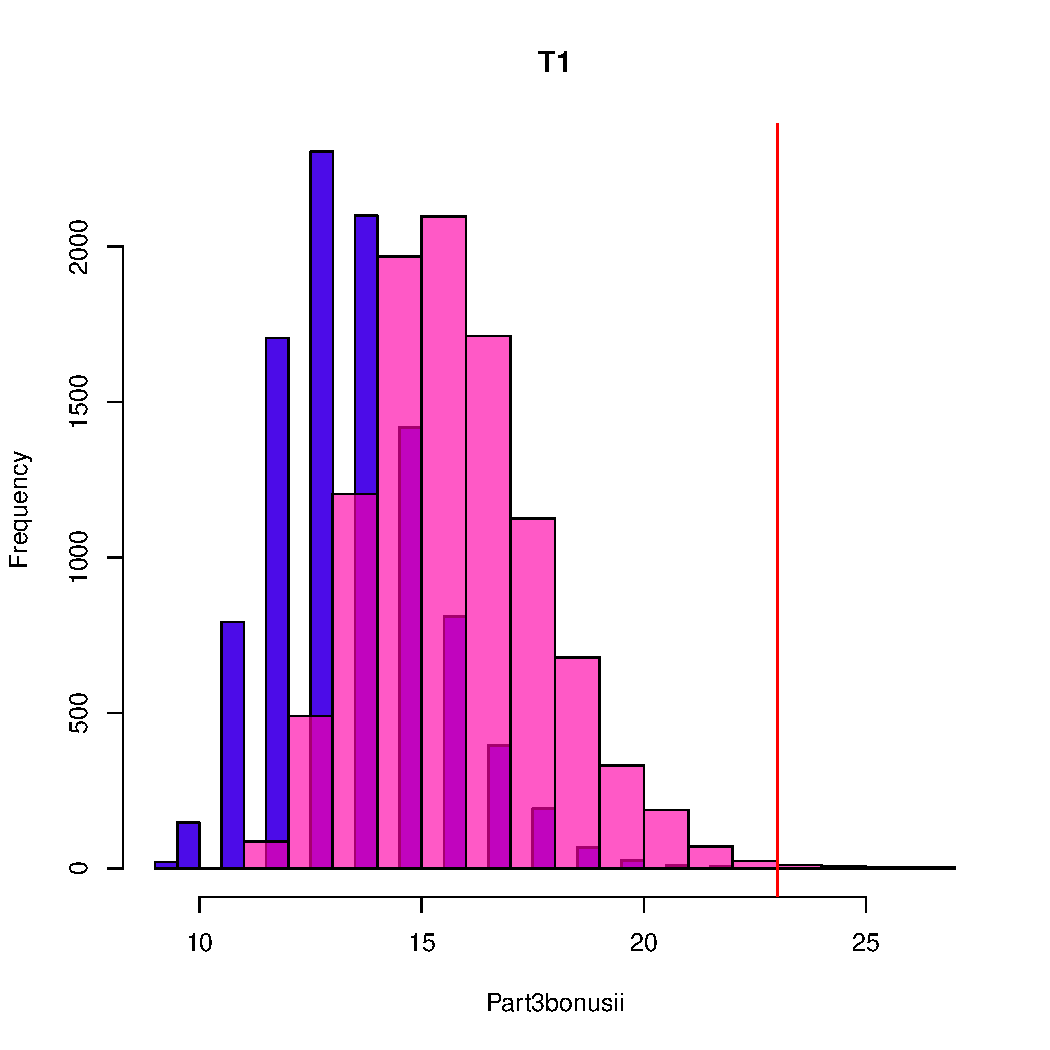
\includegraphics[width=0.33\linewidth]{figure/unnamed-chunk-11-1} 
\begin{kframe}\begin{verbatim}
# Probability of rejecting H0:
ppois(c2, mean(Part3bonusii), lower.tail = F)
## [1] 0.007217956
\end{verbatim}
\end{kframe}
\end{knitrout}

The second test $(T_2)$ has a higher probability of rejecting $H_{0}$. In order to determine this, I applied the same logic as in part b; however, I had to look at $P(X>c_{i})$ so the lower.tail needed to be set to False in pnorm. Since, the alternative is that $\lambda>10$, it should be expected that the Type I error would be small. Since $(T_{1})$ involves summing up all the values, each value is lower which helps keep the overwhelming majority of simulated sums under the value of $c_1$. 
\section*{Problem 4}
\subsection*{Part A}
\begin{knitrout}
\definecolor{shadecolor}{rgb}{1, 1, 1}\color{fgcolor}\begin{kframe}
\begin{verbatim}
EX = (mean(problem4)); MX = median(problem4); SDX = (sd(problem4))
3*(EX-MX)/SDX
## [1] 1.080882
\end{verbatim}
\end{kframe}
\end{knitrout}
For the plug in estimate, I used the the sample mean, median, and standard deviation. I computed the sample mean, median, and standard deviation, denoting them as EX, MX, and SDX repectively, then applied the formula for Pearson 2 skewness given in problem 4.
\subsection*{Part B}
\begin{knitrout}
\definecolor{shadecolor}{rgb}{1, 1, 1}\color{fgcolor}\begin{kframe}
\begin{verbatim}
bootstrap.p2s = function(){
  p4 = sample(problem4, length(problem4), replace = T)
  return(3*(mean(p4)-median(p4))/(sd(p4)))
}
bootstrap.p2sb = replicate(10000, bootstrap.p2s())
quantile(bootstrap.p2sb, c(0.05, 0.95))
##       5%      95% 
## 0.763949 1.274624
\end{verbatim}
\end{kframe}
\end{knitrout}
In order to run the bootstrap method, the first step was to create a no input function that samples the Problem4 data with replacement and then applies the Pearson 2 skewness formula. I replicated the process 10,000 times and constructed a 90\% confidence interval by using the quantile function at 5\% and 95\%.
\subsection*{Bonus}
\begin{knitrout}
\definecolor{shadecolor}{rgb}{1, 1, 1}\color{fgcolor}\begin{kframe}
\begin{verbatim}
mean(bootstrap.p2sb)-3*(EX-MX)/SDX
## [1] -0.05069033
\end{verbatim}
\end{kframe}
\end{knitrout}
There is a slightly negative bias using the bootstrap method. To calculate the Bias I did the following 
\begin{equation}
Bias_{boot}[\hat\theta^*]=E[\hat\theta^*]-\hat\theta
\end{equation}
where $E[\hat\theta^*]$ is the mean of the bootstrap distribution and $\hat\theta$ is the estimate from the orginal data.
\section*{Problem 5}
\subsection*{Part A}
\begin{knitrout}
\definecolor{shadecolor}{rgb}{1, 1, 1}\color{fgcolor}\begin{kframe}
\begin{verbatim}
mean(problem5$A==0)
## [1] 0.624
mean(problem5$A==1)
## [1] 0.376
\end{verbatim}
\end{kframe}
\end{knitrout}
These are just straight calculations from the data set with respect to column A. The mean of boolean vectors returns the percentage of the vector that is defined as TRUE by the boolean structure.
\subsection*{Part B}
\begin{knitrout}
\definecolor{shadecolor}{rgb}{1, 1, 1}\color{fgcolor}\begin{kframe}
\begin{verbatim}
mean((problem5$B[problem5$A==1])==1)
## [1] 0.5718085
mean((problem5$B[problem5$A==0])==1)
## [1] 0.2035256
\end{verbatim}
\end{kframe}
\end{knitrout}
Subsetted Column by column A to represent the subset of space, then I applied the same logic as Part A. 
\subsection*{Part C}
\begin{knitrout}
\definecolor{shadecolor}{rgb}{1, 1, 1}\color{fgcolor}\begin{kframe}
\begin{verbatim}
partC = table(problem5$B, problem5$C)
chisq.test(partC)
## 
## 	Pearson's Chi-squared test with Yates' continuity correction
## 
## data:  partC
## X-squared = 2.1224, df = 1, p-value = 0.1452
\end{verbatim}
\end{kframe}
\end{knitrout}
The cell counts for the oberved values are are greater than 5, so using the chisq.test with result in no warnings. Since the P-value of the Chi-Square for B and C is 0.1452, the null hypothesis that B and C are independent at an $\alpha=0.05$ will hold since $0.1452>0.05$. 
\subsection*{Part D}
\begin{knitrout}
\definecolor{shadecolor}{rgb}{1, 1, 1}\color{fgcolor}\begin{kframe}
\begin{verbatim}
partD = table(problem5$A, problem5$D)
chisq.test(partD)
## 
## 	Pearson's Chi-squared test with Yates' continuity correction
## 
## data:  partD
## X-squared = 1.5225, df = 1, p-value = 0.2172
\end{verbatim}
\end{kframe}
\end{knitrout}
The cell counts for the oberved values are are greater than 5, so using the chisq.test with result in no warnings. Since the P-value of the Chi-Square for A and D is 0.2172, the null hypothesis that A and D are independent at an $\alpha=0.05$ will hold since $0.2172>0.05$ 
\subsection*{Part E}
\begin{knitrout}
\definecolor{shadecolor}{rgb}{1, 1, 1}\color{fgcolor}\begin{kframe}
\begin{verbatim}
mean((problem5$D[problem5$B==1 & problem5$C==0])==1)
## [1] 0.2132701
\end{verbatim}
\end{kframe}
\end{knitrout}
The And statement corresponds to using And in the probability statement $P(D=1|B=1,C=0)$.

\end{document}
